\section*{Results} 
% \subsection*{Exclusions} 
% \begin{figure}[t]
%     \centering 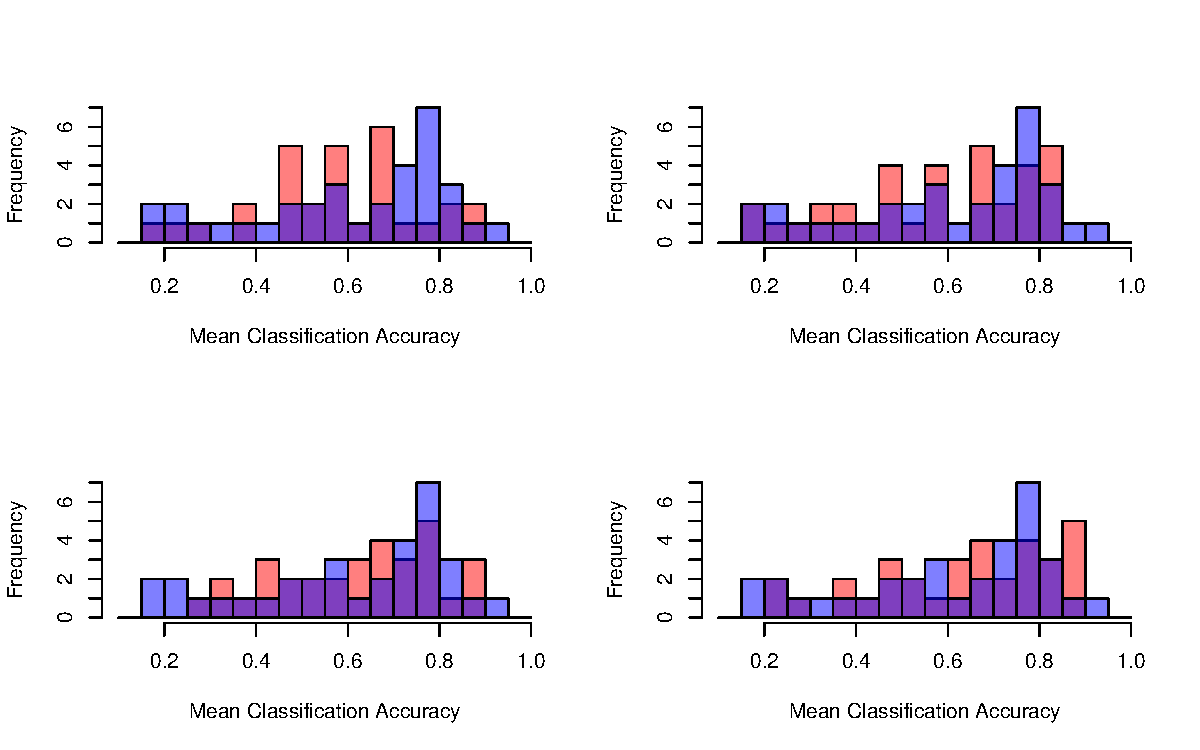
\includegraphics[width=1.0\textwidth]{../figures/fig_exc_ac.pdf}
%     \caption{
%       \textbf{A:}
%       \textbf{B:}
%       \textbf{C:}
%       \textbf{D:}
%     }
%     \label{fig:exc_acc}
% \end{figure}


\subsection*{Numerical Stroop Accuracy} 
\begin{figure}[t]
    \centering 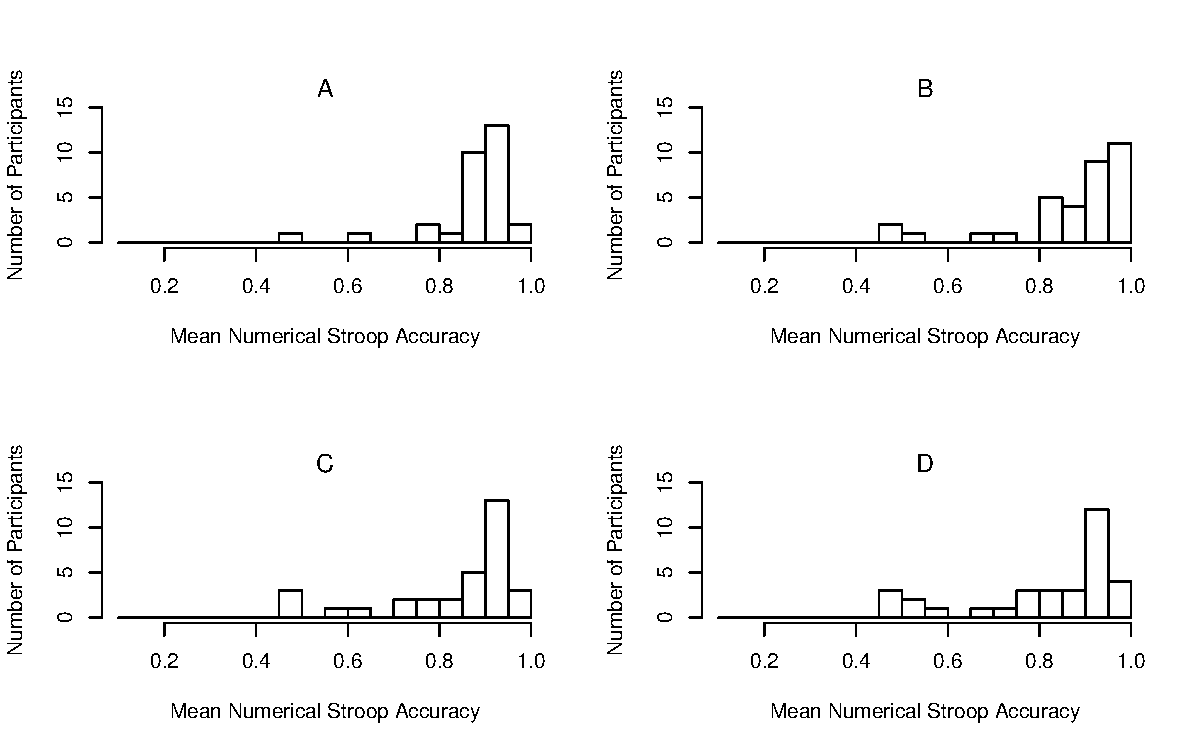
\includegraphics[width=1.0\textwidth]{../figures/fig_exc_dual.pdf}
    \caption{
      Histograms showing distribution of mean Numerical Stroop accuracy
      seperately for each condition. 
      \textbf{A:} Condition 1.
      \textbf{B:} Condition 2.
      \textbf{C:} Condition 3.
      \textbf{D:} Condition 4.
    }
    \label{fig:exc_dual}
\end{figure}

Figure \ref{fig:exc_dual} shows histograms characterizing mean dual-task performance
seperately for each condition. Overall, mean accuracy on the dual-task was very
good, with mean levels at $0.88$ in Condition 1, $0.87$ in Condition 2, $0.84$ in
Condition 3, and $0.82$ in Condition 4.

\subsection*{Classification Accuracy} 
\begin{figure}[t]
  \centering 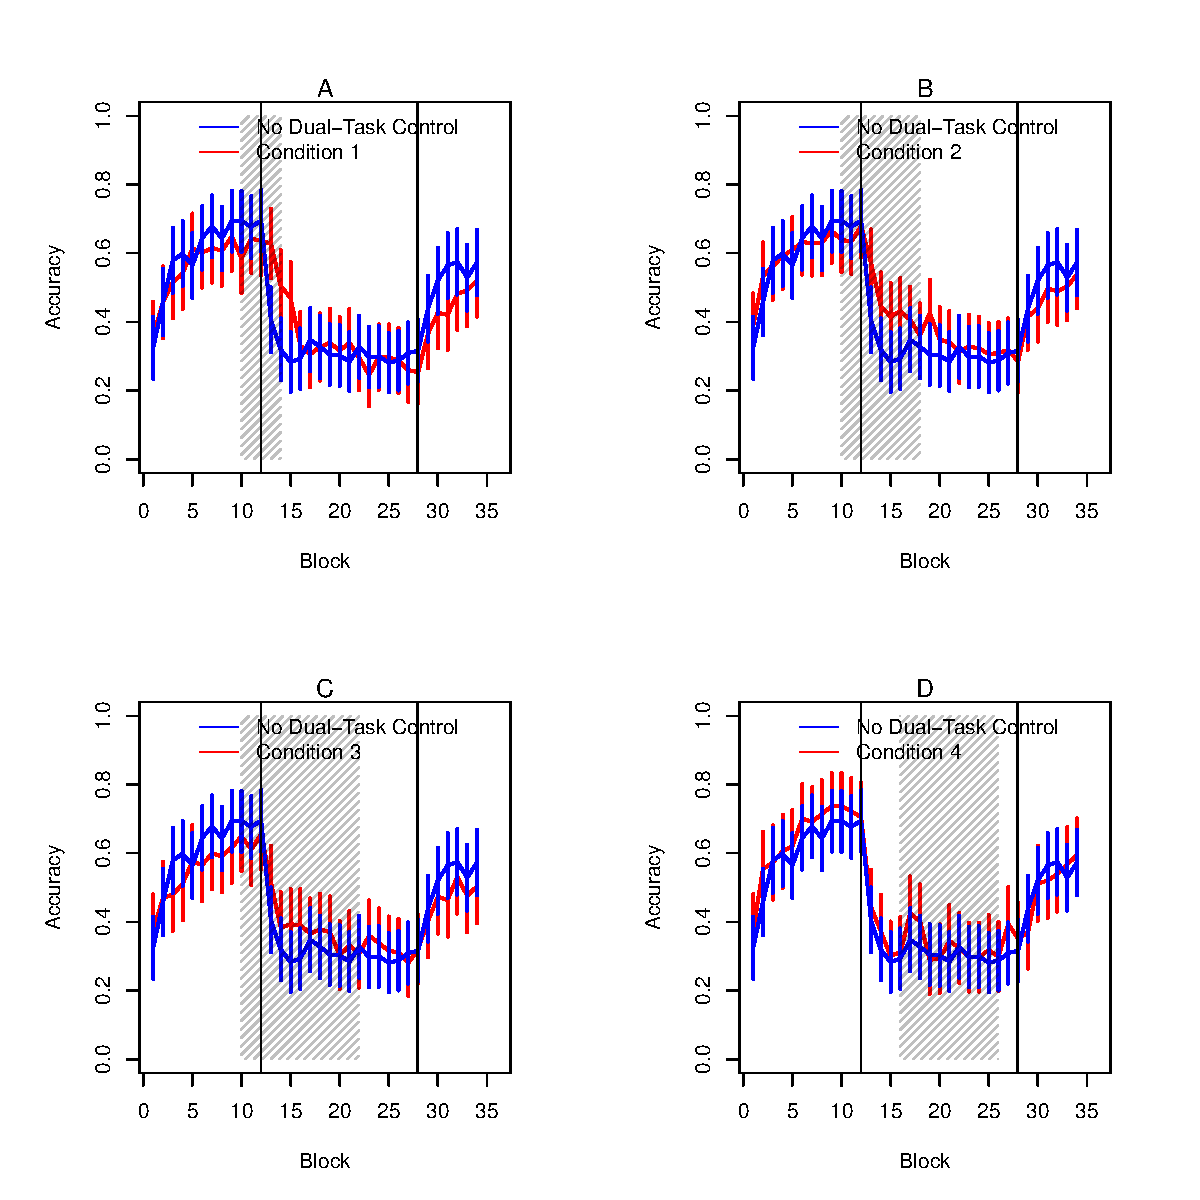
\includegraphics[width=1.0\textwidth]{../figures/fig_learning_curves.pdf}
  \caption{
    Mean accuracy per 25 trial block. The blue line in each panel is Condition
    5 (no dual-task control). The hatch marks indicate dual-task trials. The key
    features are (1) dual-task slows the change in classification strategy (seen
    in this plot as ``accuracy'' decline), and (2) the dual-task conditions show
    less savings than the no dual-task control. There is no obvious 
    dose-dependent effect of the dual task, nor is there an obvious difference
    between dual-task conditions.
    \textbf{A:} Condition 1 (dual-task applied on trial 251 through trial 350).
    \textbf{B:} Condition 2 (dual-task applied on trial 251 through trial 450). 
    \textbf{C:} Condition 3 (dual-task applied on trial 251 through trial 550). 
    \textbf{D:} Condition 4 (dual-task applied on trial 351 through trial 650). 
    Error bars are SEM.
  }
  \label{fig:learning_curves}
\end{figure}

Figure \ref{fig:learning_curves} shows the mean accuracy in each block of 25
trials across the duration of the experiment. Recall that, if feedback
contingency is computed via declarative mechanisms, then (1) dual-task trials
should slow the change in classification performance during intervention, and (2)
dual-task conditions should show reduced savings relative to the no dual-task
control. We see evidence for both features in our data.

\subsubsection*{Acquisition}
Conditions 1 through 5 are identical for the first 250 trials (10 blocks) of
acquisition (before dual-task onset), and so we expect performance during these
blocks to be the same across conditions. This is clearly the case by visual
inspection of Figure \ref{fig:learning_curves}, and is supported by the results
of a 5 Condition $\times$ 10 Block ANOVA. There was a n.s. effect of Condition
[$F(4,1620) = 1.89, p = 0.11, \Omega^2 = 0.00$], and a n.s. Condition $\times$ Block
interaction [$F(4,1620) = 1.08, p = 0.37, \Omega^2 = 0.00$]. There was a significant
effect of Block [$F(1,1620) = 191.00, p < 0.001, \Omega^2 = 0.10$], reflecting
improvement across the acquisition phase.

\subsubsection*{Intervention}
If the computation of feedback contingency is dependent on declarative
mechanisms, then we expect change in performance during intervention to be
slowed during the simultaneous performance of the Numerical Stroop. This is
clearly the case by visual inspection of \ref{fig:learning_curves}, and is
supported by the results of a 5 condition $\times$ 14 block ANOVA. A significant
effect of Condition [$F(4,2598) = 9.74, p = 0.00, \Omega^2 = 0.01$] reflected an
overall difference in intervention performance in dual-task conditions relative
to the no dual-task control. A significant effect of Block [$F(1,2598) = 166.65,
p < 0.001, \Omega^2 = 0.06$] reflected the change in classification performance
across intervention seen in all conditions. The Condition $\times$ Block
interaction was also significant [$F(4,2598) = 14.64, p < 0.001, \Omega^2 =
0.02$], reflecting the slower change in performance in the dual-task conditions
relative to the no dual-task control.

The directional interpretation of the above omnibus results is supported by
several planned comparisons. 
All dual-task conditions were significantly different from the no dual-task
control [
$condition  1 > condition  5$:
$t(940) = 2.78, p < .05, d = 0.25$;
$condition  2 > condition  5$:
$t(1046) = 5.31, p < .01, d = 0.87$;
$condition  3 > condition  5$:
$t(962) = 5.45, p < .01, d = 0.96$;
$condition  4 > condition  5$:
$t(996) = 2.99, p < .01, d = 0.28$;
].
The effect of the dual-task during intervention required the dual-task during
the acquisition-intervention phase transition [
$condition  2 > condition  4$:
$t(1063) = 1.94, p = 0.05, d = 0.12$;
$condition  3 > condition  4$:
$t(1037) = 2.24, p = 0.03, d = 0.16$;
],
Although there was no difference between condition 1 (shortest dual-task
exposure) and condition 4 [
$condition  1 > condition  4$:
$t(1006) = -0.23, p = 0.82, d = 0.00$;
].

\subsubsection*{Savings: Group Level} 
\begin{figure}[t]
  \centering 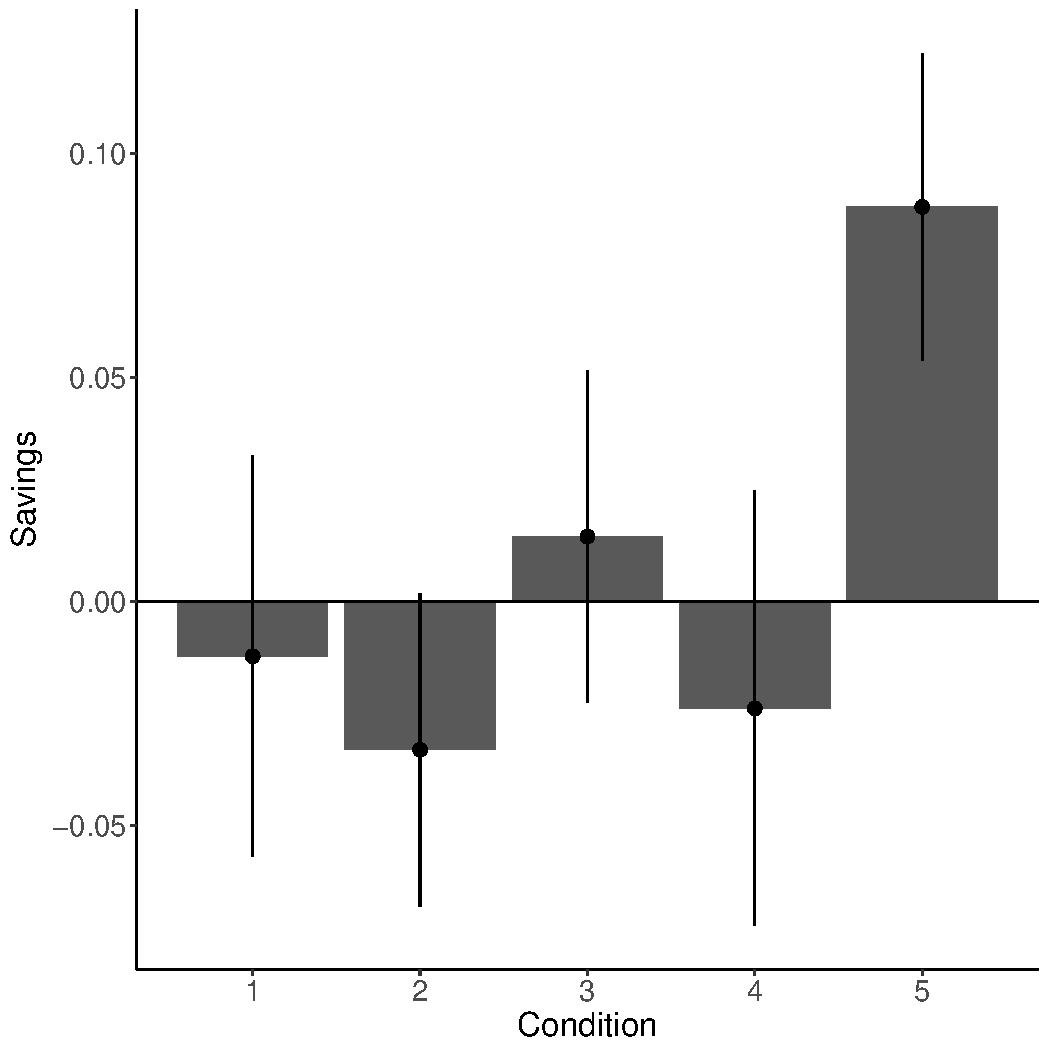
\includegraphics[width=1.0\textwidth]{../figures/fig_savings.pdf}
  \caption{
    savings (mean of all 150 reacquisition trials - mean of the first 150
    acquisition trials) in all conditions of the present experiment, and also
    including data from crossley et al. (2013), which shows the savings observed in
    a no dual-task control condition with only 300 trials of intervention. each
    circle corresponds to a single subject.
  }
  \label{fig:savings}
\end{figure}

\begin{figure}[t]
  \centering 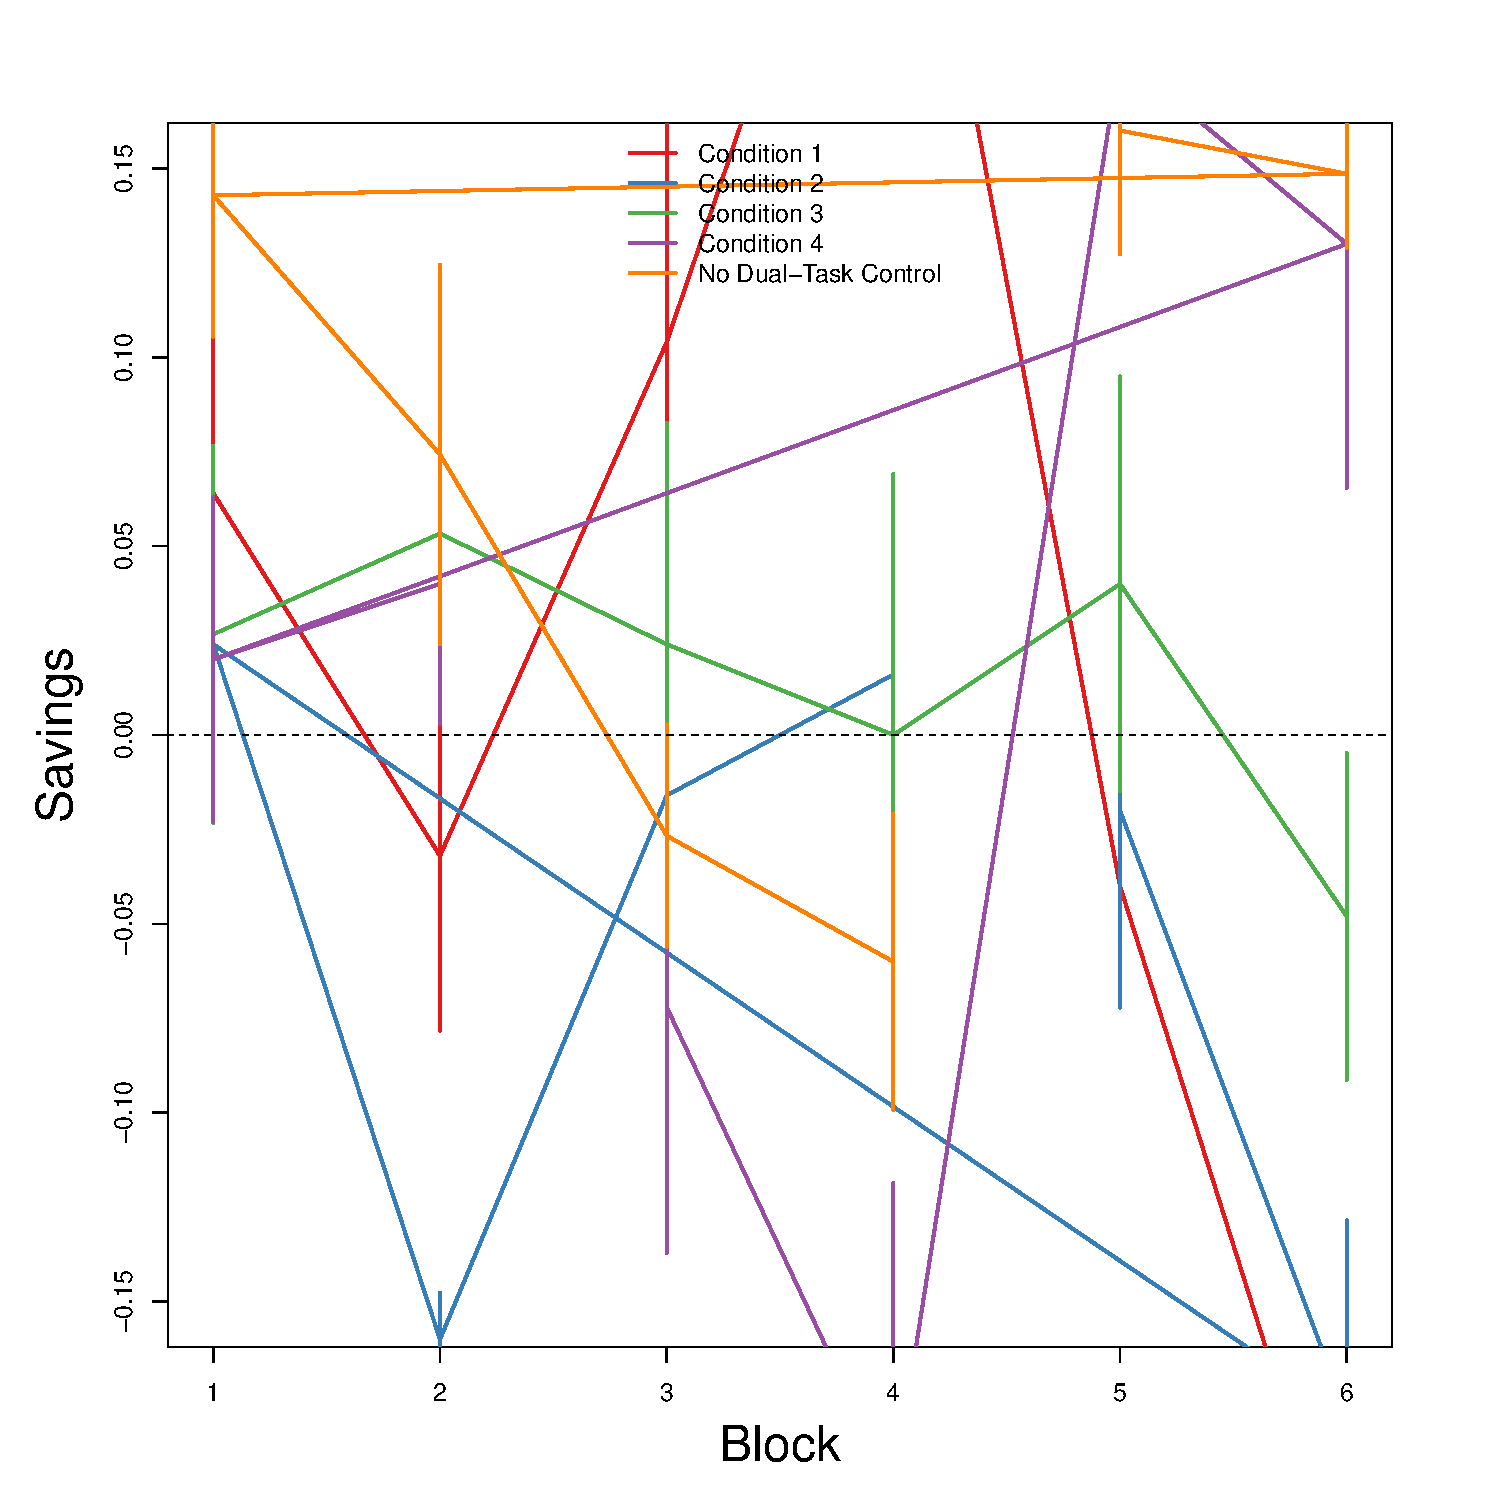
\includegraphics[width=1.0\textwidth]{../figures/fig_savings_per_block.pdf}
  \caption{
    Savings (reacquisition - acquisition) per 25 trial block. 
    Error bars are SEM. 
  }
  \label{fig:savings_per_block}
\end{figure}

If the computation of feedback contingency depends on declarative systems, then
we expect the dual-task conditions to exhibit less savings than the no dual-task
control. This is apparent via visual inspection of Figure
\ref{fig:learning_curves} (e.g., the red lines are always below the blue line),
and also of Figure \ref{fig:savings}, which shows the savings observed for every
participant in every condition as a box plot with individual subject data points
superimposed. Inpection of Figure \ref{fig:savings_per_block} reveals that
savings is greatest at the beginning and gradually declines. Savings in the no
dual-task control condition is significantly greater than in any other
condition. In fact, positive savings is not reliably expressed in any dual-task
condition, even on block 1, and quickly reflects negative savings (interference:
relearning worse than initial learning) in later blocks. These observations are
supported via the results of a 5 condition $\times$ 6 block ANOVA. There was a
significant effect of Condition [$F(1,974) = 5.77, p < 0.05, \Omega^2 = 0.01$],
indicating less savings in the dual-task condition relative to the no dual-task
condition. There was a significant effect of Block [$F(1,974) = 22.55, p <
0.001, \Omega^2 = 0.02$], indicating that savings in all conditions was most
prominent during early blocks and gradually tapered off (see Figure
\ref{fig:savings_per_block}). The Condition $\times$ Block interaction was n.s.
[$F(1,974) = 0.001, p = 0.97, \Omega^2 = 0.00$].
    
The directional interpretation of the above omnibus results is supported by
several planned comparisons. 
Condition 2 savings are significantly less than condition 5 [$t(63) = -2.09, p =
0.04, d = 0.55$].
Savings in the remaining dual-task conditions were all marginally less than
condition 5 [
$condition  1 > condition  5$:
$t(46) = -1.24, p = 0.22, d = 0.22$;
$condition  3 > condition  5$:
$t(57) = -1.63, p = 0.11, d = 0.35$;
$condition  4 > condition  5$:
$t(61) = -1.67, p = 0.10, d = 0.36$;
].
There were no significant differences in savings between any dual-task condition [
$condition  1 > condition  2$:
$t(53) = 0.37, p = 0.71, d = 0.02$;
$condition  1 > condition  3$:
$t(56) = 0.12, p = 0.90, d = 0.00$;
$condition  1 > condition  4$:
$t(53) = 0.08, p = 0.94, d = 0.00$;
$condition  2 > condition  3$:
$t(63) = -0.29, p = 0.78, d = 0.01$;
$condition  2 > condition  4$:
$t(65) = -0.36, p = 0.72, d = 0.02$;
$condition  3 > condition  4$:
$t(62) = -0.06, p = 0.96, d = 0.00$;
].

\subsubsection*{Savings: Subject Level} 
\begin{figure}[t]
  \centering 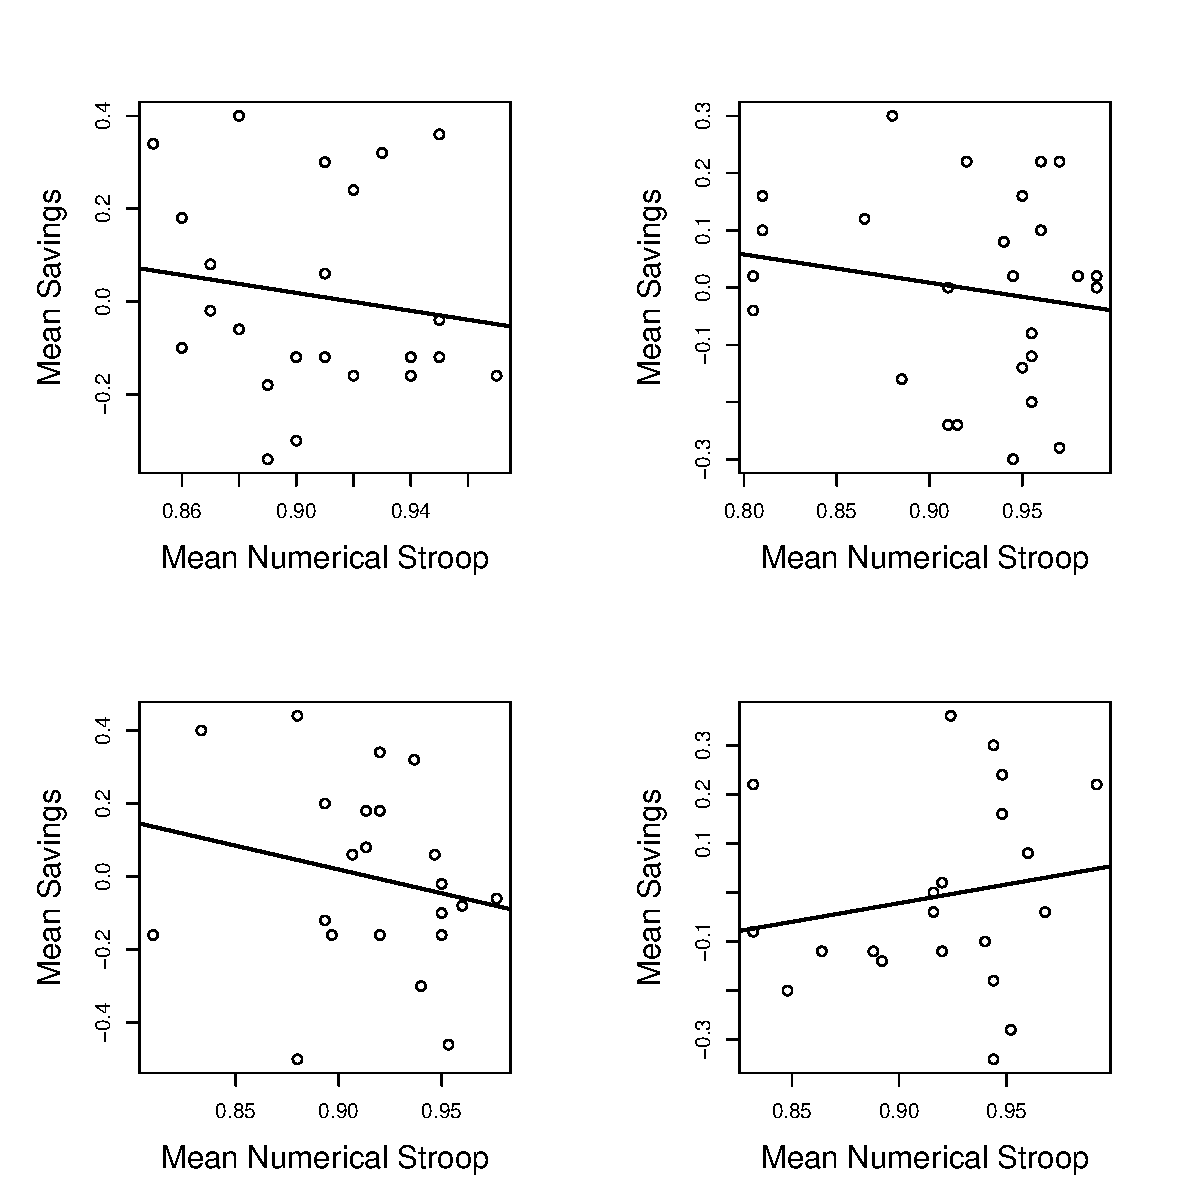
\includegraphics[width=1.0\textwidth]{../figures/fig_savings_dt.pdf}
  \caption{
    Does dual-task performance predict savings?
  }
  \label{fig:savings_dt}
\end{figure}

\begin{figure}[t]
  \centering 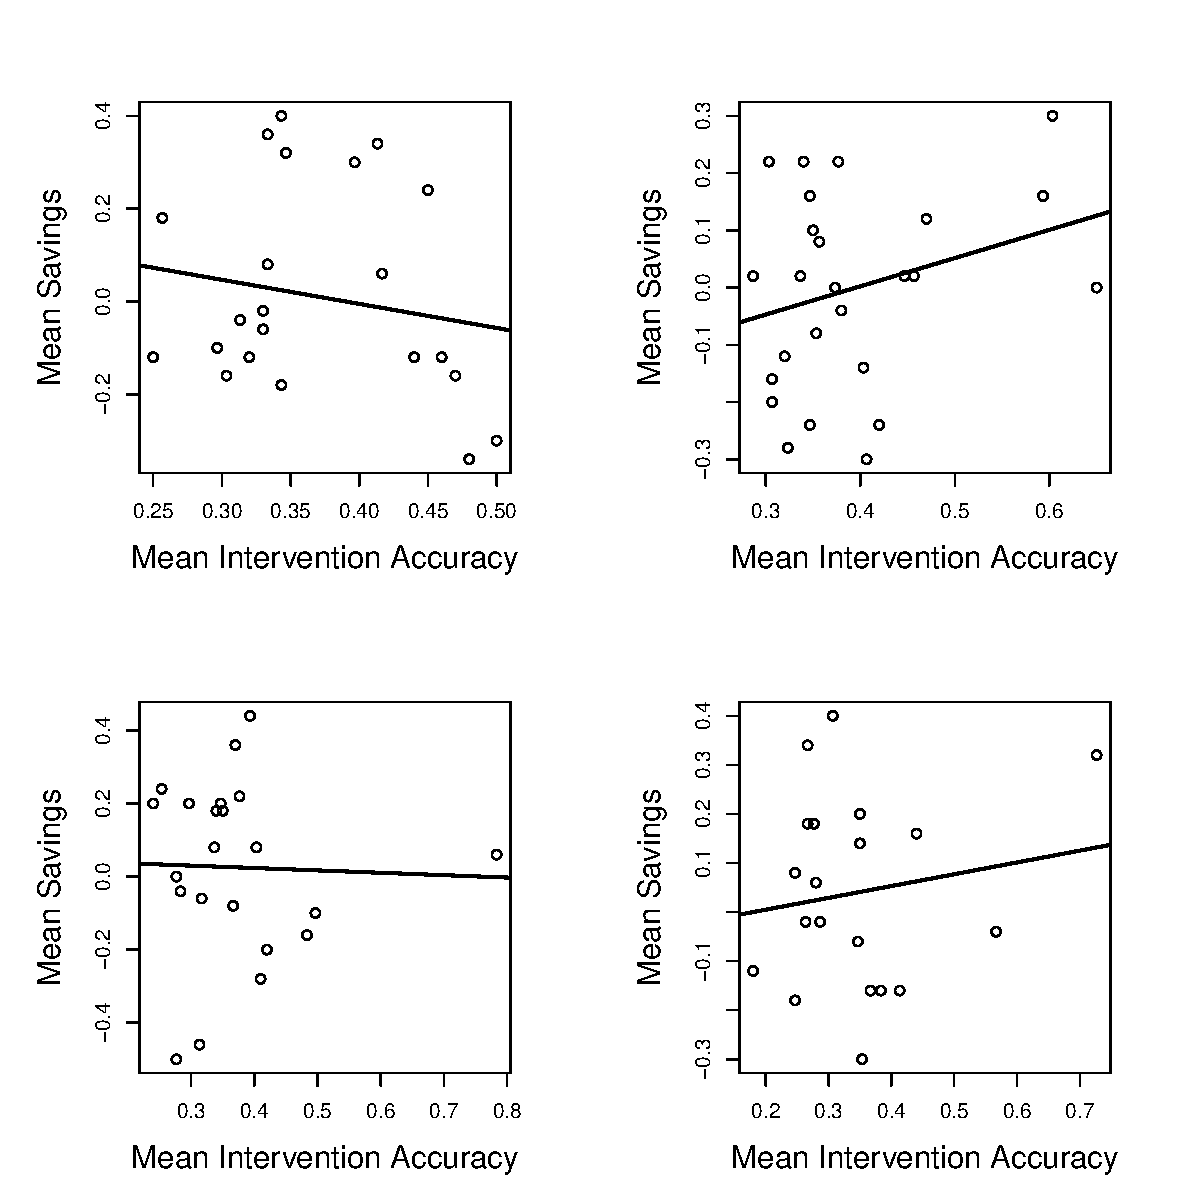
\includegraphics[width=1.0\textwidth]{../figures/fig_savings_int.pdf}
  \caption{
    Does dual-task performance predict savings?
  }
  \label{fig:savings_int}
\end{figure}

\begin{figure}[t]
  \centering 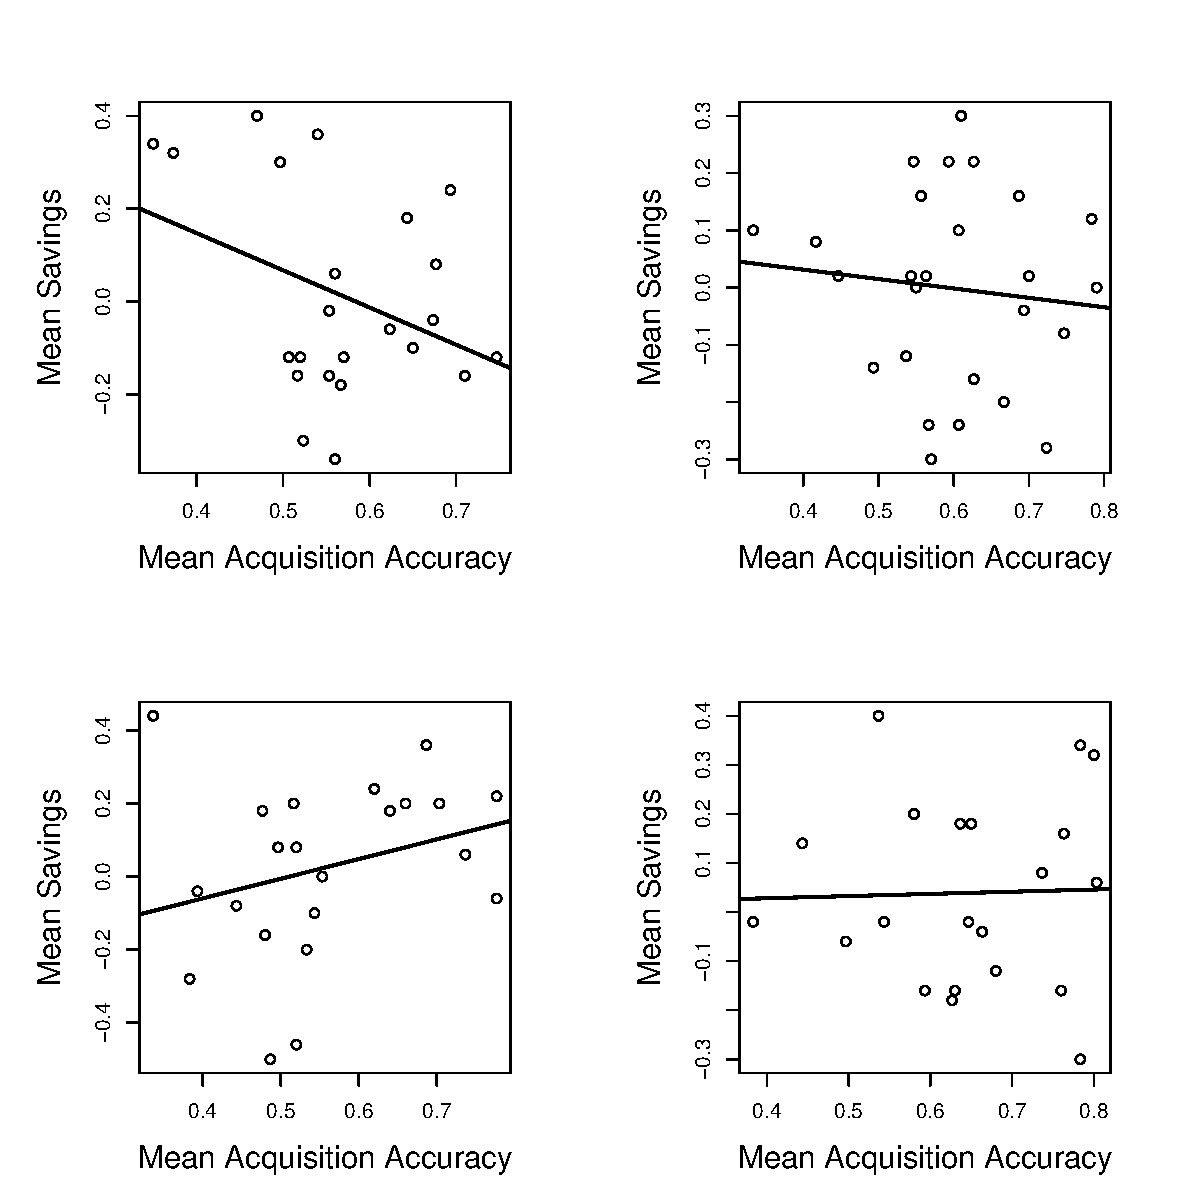
\includegraphics[width=1.0\textwidth]{../figures/fig_savings_ac.pdf}
  \caption{
    Does dual-task performance predict savings?
  }
  \label{fig:savings_ac}
\end{figure}

Figure \ref{fig:savings} shows high variability with many subjects in all
condtions expressing both postitive and negative savings. This sections presents
the results of an exploratory analysis asking what factors might predict savings
in the indivudal subject. We performed a series of simple linear regressions to
examine the effect of (1) mean dual-task accuracy, (2) mean intervention
accuracy, and (3) mean acquisition accuracy.

Our first thought was that dual-task performance might reflect the degree to
which the computation of feedback contingency might be impaired, and thereby
predict savings. Figure \ref{fig:savings_dt} shows that this is not the case.
Mean dual-task performance was not predictive of savings in any condition. 

We next explored the idea that mean accuracy during intervention may predict
savings. The rationale here is that mean intervention accuracy may reflect the
degree to which procedural knowledge is being expressed, and therefore is
vulnerable to modification. Figure \ref{fig:savings_int} shows that mean
intervention accuracy was not predictive of savings in any condition.

The final idea we explored was that mean acquisition accuracy may predict
savings. The intuition here is that the stronger intitial learning, the more
robust to intervention it may be, and the more likely it should be manifest as
savings in relearning. Figure \ref{fig:savings_ac} shows that mean acquisition
accuracy does not predict savings in any condition.

% \subsection*{Decision-Bound Modeling} 
% \begin{figure}[t]
%   \centering 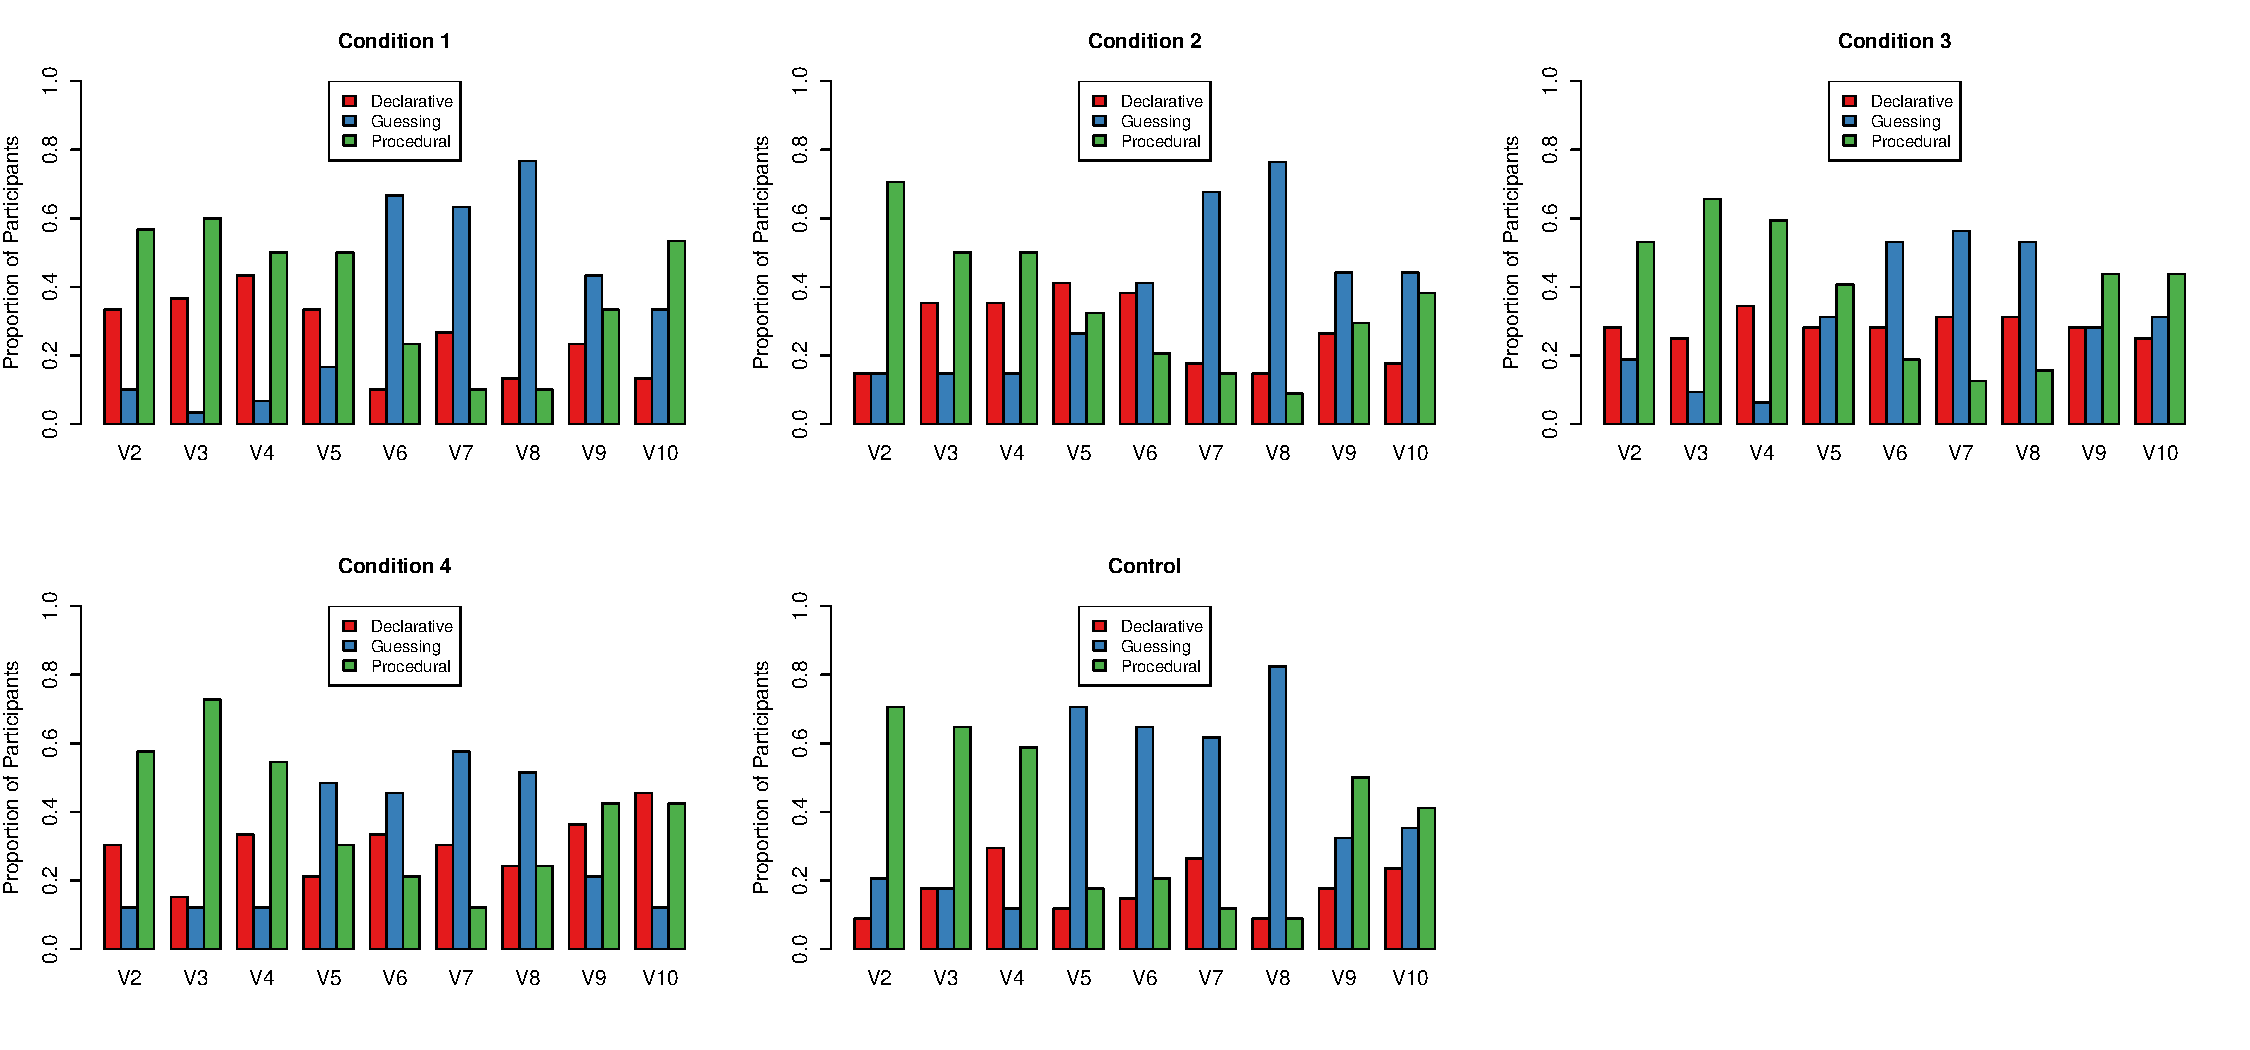
\includegraphics[width=1.0\textwidth]{../figures/fig_model_fits.pdf}
%   \caption{
%     Proportion of participants best fit by a decision-bound model assuming a
%     procedural, declarative, or guessing strategy. The key feature of this
%     figure is that participants in the no dual-task control condition changed
%     their response strategy more during the intervention more quickly than
%     participants in all dual-task conditions. 
%     \textbf{A:} Condition 1 (dual-task applied on trial 251 through trial 350).
%     \textbf{B:} Condition 2 (dual-task applied on trial 251 through trial 450). 
%     \textbf{C:} Condition 3 (dual-task applied on trial 251 through trial 550). 
%     \textbf{D:} Condition 4 (dual-task applied on trial 351 through trial 650). 
%     \textbf{E:} Condition 5 (no dual-task control). 
%   }
%   \label{fig:exp_fits}
% \end{figure}
